\documentclass[12pt,a4paper]{scrartcl}

%Schriftart
\usepackage{helvet}
\renewcommand{\familydefault}{\sfdefault}

%Zeilenabstand
\usepackage{setspace}
\onehalfspacing

%Packages
\usepackage[utf8]{inputenc}
\usepackage[T1]{fontenc}
\usepackage[english,ngerman]{babel}
\usepackage{mathrsfs}
\usepackage[pdftex]{graphicx}
\usepackage{latexsym}
\usepackage{amsmath,amssymb,amsthm}
\usepackage{geometry}
\usepackage{enumitem}   
\usepackage[LGRgreek]{mathastext}
\usepackage{mathtools}


%Geometrie der Blätter
\geometry{a4paper, top=40mm, left=30mm, right=30mm, bottom=30mm,
headsep=10mm, footskip=12mm}
\setlength{\topmargin}{0mm}

%Mathematische Werkzeuge
\newtheorem{Satz}{Satz}[section]
\newtheorem{Definition}[Satz]{Definition} 
\newtheorem{Lemma}[Satz]{Lemma}		   
\newtheorem{Bemerkung}[Satz]{Bemerkung}
\newtheorem{Beispiel}[Satz]{Beispiel}
\newtheorem{Annahme}{Annahme}
\numberwithin{equation}{section} 

% einige Abkuerzungen
\newcommand{\C}{\mathbb{C}} 
\newcommand{\K}{\mathbb{K}} 
\newcommand{\R}{\mathbb{R}} 
\newcommand{\Q}{\mathbb{Q}} 
\newcommand{\Z}{\mathbb{Z}} 
\newcommand{\N}{\mathbb{N}}

% einige Verbesserungen
\renewcommand{\hat}[1]{\widehat{#1}}


\begin{document}
\pagestyle{empty}
\pagenumbering{Roman} 


%%%%%%%%%%%%%%%%%%%%%%%%%%%%%%%%%%%%%%%%%%%%%%%%%%%%%%%%%%%%%%%%%%


% Titelblatt der Arbeit
\begin{titlepage}

\vspace*{1cm} 
\begin{center} 


\textbf{\Huge Präkonditionierer für zell-basierte finiten Elemente Operatoren} 
\vspace*{2cm}

{\Large Bachelorarbeit}
\vspace*{1cm}


eingereicht von \\[0.5cm]

{\Large Enes Witwit}
\vspace*{1cm}

betreuut von  \\[0.5cm]
{\Large Prof. Dr. Kanschat}
\vspace*{3cm}

\textbf{
Fakultät für Mathematik und Infromatik\\[1cm]
Universität Heidelberg}
\end{center}
\end{titlepage}

%%%%%%%%%%%%%%%%%%%%%%%%%%%%%%%%%%%%%%%%%%%%%%%%%%%%%%%%%%%%%%%%%%


\newpage
\thispagestyle{empty}
\vspace*{14cm}

\noindent\rule{16cm}{0.4pt}

Hiermit versichere ich, dass ich die vorliegende Bachelorarbeit selbständig
verfasst habe.
Ich versichere, dass ich keine anderen als die angegebenen Quellen benutzt und
alle wörtlich oder sinngemäß aus anderen Werken übernommenen Aussagen als
solche gekennzeichnet habe, und dass die eingereichte Arbeit weder vollständig
noch in wesentlichen Teilen Gegenstand eines anderen Prüfungsverfahren
gewesen ist. \\[2ex] 

\noindent

\today \hspace*{1cm}  Heidelberg \hspace*{5cm} Unterschrift\\[5ex]
% Unterschrift (handgeschrieben)

%%%%%%%%%%%%%%%%%%%%%%%%%%%%%%%%%%%%%%%%%%%%%%%%%%%%%%%%%%%%%%%%%%

\newpage
Zusammenfassung



%%%%%%%%%%%%%%%%%%%%%%%%%%%%%%%%%%%%%%%%%%%%%%%%%%%%%%%%%%%%%%%%%%

%Inhaltsverzeichnis
\newpage
\tableofcontents


 
%%%%%%%%%%%%%%%%%%%%%%%%%%%%%%%%%%%%%%%%%%%%%%%%%%%%%%%%%%%%%%%%%%


\newpage
\section*{Notation}
\addcontentsline{toc}{section}{Notation}



%%%%%%%%%%%%%%%%%%%%%%%%%%%%%%%%%%%%%%%%%%%%%%%%%%%%%%%%%%%%%%%%%%




\newpage
\section*{Abbildungsverzeichnis}
\addcontentsline{toc}{section}{Abbildungsverzeichnis}
\listoffigures


%%%%%%%%%%%%%%%%%%%%%%%%%%%%%%%%%%%%%%%%%%%%%%%%%%%%%%%%%%%%%%%%%%



\newpage
\section*{Tabellenverzeichnis}
\addcontentsline{toc}{section}{Tabellenverzeichnis}

%%%%%%%%%%%%%%%%%%%%%%%%%%%%%%%%%%%%%%%%%%%%%%%%%%%%%%%%%%%%%%%%%%


% Ab sofort Seitenzahl in Fußzeile
\newpage
\pagestyle{plain}


%%%%%%%%%%%%%%%%%%%%%%%%%%%%%%%%%%%%%%%%%%%%%%%%%%%%%%%%%%%%%%%%%%

\pagenumbering{arabic} 
\setcounter{page}{1}
%Einleitung und Motivation
\section{Einführung}
Hochleistungsrechnen ist eine neue Disziplin, die mit dem Drang entstand, immer komplexere Probleme zu lösen. Diese neue Art an Probleme ranzugehen, löst sie nicht. Doch sie eröffnet uns eine neue Sichtweise auf dasselbe Probleme und gibt uns am Ende womöglich neue Lösungsansätze.
Parallelisierung ist ein großer Zweig des Hochleistungsrechnens. Das Grundgerüst dieser Methodik besteht darin komplexe Probeme modular zu lösen, das heißt sie in viele wenig komplexere Subprobleme zu unterteilen, die unabhängig voneinander berechenbar sind. Am Ende fasst man die Ergebnisse der Subprobleme zu einem Ergebnis zusammen, welches die Lösung des komplexen Problems darstellt.

\begin{equation} \label{eq:main}
v=A(u)=\sum_{k=1}^{n_{cells}} C^T P_k^T A_k (P_k Cu)
\end{equation}

ist die Gleichung, welche wir mit Hilfe der finite Elemente Methode lösen wollen. A ist ein möglicherweise nichtlinearer Operator, der Vektor u als Input nimmt und das Integral vom Operator multipliziert mit  Testfunktionen $\phi_i$ mit $i=1,\dots,n$, berechnet ~\cite[136]{Kronbichler}. Damit wir diese Gleichung besser nachvollziehen können, werden wir sie im nächsten Kapitel herleiten. Doch um diese Arbeit zu motivieren kann man sich diese Gleichung so vorstellen, dass man ein großes Problem in eine Summe von kleineren Problemen unterteilt. 

Nun die Matrix $A_k$ kann durchaus, wie wir nachher erkennen werden, sehr groß werden. Wenn sie so groß wird, dass sie nicht mehr im Cache liegt, bekommen wir das Problem, dass der Zugriff auf Elemente der Matrix sehr teuer wird. Dementsprechend wollen wir uns vorallem bei der Herleitung unserer Methoden um diese Subprobleme zu lösen auf sogenannten matrix-freie Heransgehensweisen konzentrieren. Das bedeutet wir wollen nicht explizit die Matrix $A_k$ ausrechnen, sondern stattdessen ihre Elemente dort berechnen wo sie auch gebraucht werden. Ob dies möglich ist, ist für diese Arbeit von großer Bedeutung. 

Der Sinn dieser Arbeit ist einen effiziente Ansatz herzuleiten, der uns 

\begin{equation} \label{eq:main2}
A_k^{+}v_k
\end{equation}

berechnet, wobei $A_k^{+}$ eine Pseudoinverse darstellt. Dies kann als Präkonditionierer genutzt werden, um (\ref{eq:main}) Gleichung zu lösen. Das heißt die Resultate dieser Arbeit werden benutzt, um damit einen Präkonditionierer zu bauen. Daraus folgern wir, dass die Exaktheit der Lösung von (\ref{eq:main2}) eine redundante Rolle spielt, vielmehr sollten wir eine optimale Lösung im Trade-Off zwischen Genauigkeit und Komplexität anstreben.

Im zweiten Kapitel werden wir erstmal en theoretisches Grundgerüst schaffen, um die beiden Gleichungen besser zu durchleuchten und nachvollziehen zu können. Wir werden uns die Grundlagen der numerischen Behandlung von partiellen Differentialgleichungen anschauen und versuchen die oberen Gleichungen herzuleiten.
Im zweiten Teil des zweiten Kapitels werden wir uns mit Tensor Dekomposition beschäftigen. Dies liegt daran, dass wir uns den Operator A als Tensor umdefinieren können und die Pseudoinverse mit Hilfe der sogenannten Singulärwertzerlegung höherer Ordnung berechnen können.

Im dritten Kapitel werden wir uns zwei Methoden anschauen die Pseudoinverse zu berechnen. In der erste Methode die Struktur des Operators A zu nutze und leiten eine Repräsentation von A her die uns die Pseudoinverse mit wenig Aufwand gibt. In der zweiten Methode werden wir uns wie bereits erwähnt, A als Tensor umdefinieren und versuchen die SIngulärwertzerlegung höherer Ordnung effizient zu berechnen und uns dort auch Strukturen vom Tensor zu nutze zu machen.

Im vierten Kapitel sprechen wir über die effiziente Implementierung beider Algorithmen und im fünften Kapitel fassen wir alle Resultate zusammen und schließen mit einem Fazit ab.







%\input{./Einleitung/motivation.tex}



%%%%%%%%%%%%%%%%%%%%%%%%%%%%%%%%%%%%%%%%%%%%%%%%%%%%%%%%%%%%%%%%%%


% Chapter 1
\section{Theorie}
\subsection{Schwache Lösungen}
Es ist naheliegend, dass wir uns zu erst mit notwendigen Funktionenräumen beschäftigen und uns auf analytischer Ebene eine Umformulierung der Differentialgleichung zu nutze machen, welche uns letztlich die Grundlage für die finiten Elementen Methode liefert.

Dazu schauen wir uns folgendes Randwert Problem an:
\begin{equation}
	- \Delta u = f \text{ in } \Omega	
\end{equation}

Wir sehen von der Form der Differentialgleichung, dass die gesuchte \textit{klassische Lösung}, was immer das auch bedeuten mag, bestimmte Bedingungen zu erfüllen hat. Nämlich, dass $u$ zweimal differenzierbar sein sollte.
Ein funktionalanalytischer Ansatz versucht nun die Räume zu definieren, in der die Lösung $u$ liegt. In unserem Fall wäre folgender Raum ergiebig:

\begin{equation*}
	H^{1}(\Omega) = \{ v \in L_{2}(\Omega) : \dfrac{\delta v}{\delta x_{i}} \in L_{2}(\Omega), i=1,...,d \}
\end{equation*}

Diese Räume nennt man Sobolev Räume. Allgemein sind sie definiert durch:

\begin{Definition} Sobolev-Raum

\end{Definition}

Von der analytischen Perspektive ist die Wahl des Funktionenraumes essentiell für den Nachweis der Existenz der Lösung. Von der Perspektive der finiten Elementen Methode ist dies für die Fehlerabschätzung wichtig, da wir dann die induzierte Norm des Funktionenraumes benutzen~\cite[36]{Johnson}. Beide genannten Themen würden den Rahmen dieser Bachelorarbeit sprengen, daher verweis ich an gegebenen Stellen an weiterführende Literatur.


\subsection{Methode der finiten Elemente}
% Einführing in die FEM mit Hilfe von Grossman S.175
Im vorherigen Kapitel haben wir das \textit{Galerkin Verfahren} kennengelernt. Der Kernaspekt dieser konformen Approximation war eine Diskretisierung des Raumes und damit einhergehend global einheitlich definierte Basisfunktionen des diskreten Raumes. Nun öffnen wir die zuletzt genannte Einschränkung und fordern nur noch stückweise definierte Funktionen. Wo genau eine Funktion, in der Regel ein Polynom, definiert ist, hängt von unsererer Gebietszerlegung ab.
Das heißt für die \textit{finite Elemente Methode (FEM)} sind folgende Schritte nötig:
\begin{enumerate}
\item Das Grundgebiet in geometrisch einfache Teilgebiete $ \, \Omega_h = \, \{ \, \Omega_k \, \}_{k=1 \, , \dots, \, N} \, $ zu unterteilen, zum Beispiel Dreiecke und Rechtecke bei Problemen in der Ebene oder Tetraeder und Quader bei Problemen im dreidimensionalen Raum.
\item Definition von Ansatz- und Testfunktionen über Teilgebieten 
\item Da wir zwischen den Teilgebieten eine Stetigkeit fordern, definiert man Übergangsbedigungen, die uns globale Stetigkeit sichern
\end{enumerate}
Die Stetigkeit der globalen Lösung wird gefordert, damit wir $V_n \subset V$ bekommen, mit V ein Sobolev Raum.\cite[175]{Numerik}. 

% Voraussetzungen an die Gebietszerlegung

\begin{Bemerkung} (Voraussetzungen an Zerlegung) \cite[176]{Numerik} \\
Die Voraussetzungen an die Zerlegung $Z \, = \, \{  \, \Omega_j  \, \}_{j=1}^{m} \, $ sind 
\begin{enumerate}
\item \, \, $\bar{\Omega} \, = \,  \bigcup\limits_{j=1}^{m} \, \bar{\Omega_j}  $
\item  \, \, $int (\Omega_i) \, \cap \, int (\Omega_j) \, = \,  \emptyset  \, \, \, \text{ , falls } i \neq j $
\end{enumerate}
\end{Bemerkung}

\newpage
% Beispiel
\begin{Beispiel} 
E sei $\Omega = [a,b]$. Wir definieren Gitterpunkte $\, \{ \, x_i \, \}_{i=0}^{N} \, $ über $\, \bar\Omega \, $  beschrieben wie folgt
\begin{equation*}
a = x_0 < x_1 < x_2 < \dots < x_{N-1} < x_N = b
\end{equation*}
und eine Zerlegung  $\, Z= \, \{ \, \Omega_j  \, \}_{j=1}^{m} \, $ mit $ \, \Omega_i \, := \,  ( \, x_{i-1} \, , \, x_i \,)$ für $\, \, \, i \, = \,1 \, , \, \dots \, , \, N$. 
Ferner sei $\, h_i := x_i - x_{i-1} \, \, , \, \,  i=1,\dots,N$. Wir wählen lineare Ansatzfunktionen $ \, V_h=lin \, \{ \, \varphi_i \, \}_{i=0}^{N} \,$, wobei die Ansatzfunktionen durch
\begin{equation*}
\begin{aligned}
\varphi_i(x) \, \, &= \, 
\begin{cases}
\, \, \, \, \dfrac{1}{h_i} \, \, \, \, (x-x_{i-1})   \, \, \, \, \, \,  \text{ für } x \in \Omega_i \\
\, \, \dfrac{1}{h_{i+1}} \, (x_{i+1}-x) \, \, \, \, \, \text{ für } x \in \Omega_{i+1}  \\
\, \, \, \, \, \,  0 \, \, \, \, \, \, \, \, \,  \, \, \, \, \, \, \, \, \, \, \, \, \, \, \, \, \, \, \, \, \, \, \, \, \, \, \, \text{ sonst }
\end{cases}
\end{aligned}
\end{equation*}

definiert sind. Es gilt nach Konstruktion $\, \varphi \in C(\, \bar{\Omega} \, )$ sowie $\, \varphi_{i}\mid_{\Omega_{j}} \in C^{1}(\bar{\Omega_{j}})$, somit hat man insgesamt $\varphi_i \in H^{1}(\Omega)$ \cite[184]{Numerik}.
Die folgende Abbildung stellt die Graphen von Ansatzfunktionen $\varphi_i$ dar.

\begin{figure}[ht]
	\centering
  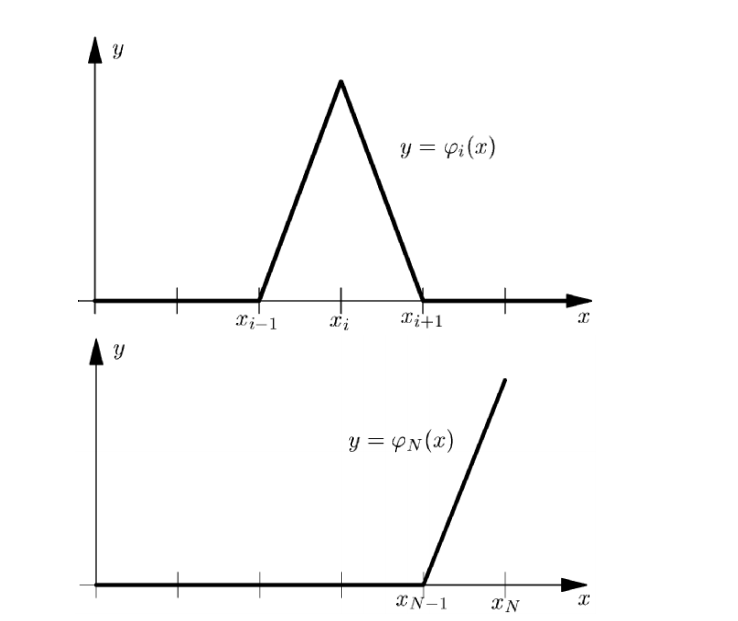
\includegraphics[width=0.6\textwidth]{hatfunction.png}
	\caption{Ansatzfunktionen $\varphi_i$ \cite[184]{Numerik}}
	\label{fig:hat}
\end{figure}

Es gilt demnach $\, \, \varphi_i (x_k) = \delta_{ik}$ mit  $\, i  ,  k = \, 0 \, , \, 1 \, , \, \dots \,, \,N \,$.
\end{Beispiel}

Nun haben wir eine Vorstellung davon, wie man ein Gebiet zerlegt, wie Ansatzfunktionen aussehen könnten und welche Eigenschaften sie zu erfüllen haben. Doch wie genau sieht das diskrete Problem bei der \textit{finite Elemente Methode} aus? Dazu müssen wir uns die sogenannte \textit{Assemblierung} der \textit{Steifigkeitsmatrix} $A_n$ anschauen. Wir werden uns die Teilelemente der Zerlegung dazu einzeln anschauen und sogenannte \textit{Elementsteifigkeitsmatrizen} ausrechnen. Im \textit{Assemblierungsschritt} werden wir dann die  \textit{Elementsteifigkeitsmatrizen} zur \textit{globalen Steifigkeitsmatrix} zusammensetzen.
Wir werden hier nodale Basisfunktionen benutzten. Diese sind durch $\, \varphi_k \, ( \, x_l \, ) = \delta_{kl} \,$ definiert. Weiterhin sei $N$ die Anzahl der Freiheitsgrade. Rekapitulieren wir das zu lösende Problem:

\begin{framed}
\begin{enumerate}
\item $
\text{ Finde ein } u_n \in V_n \text{ : } a(u_n,v_n) = f(v_n) \text{ für alle } v_n \in V_n
$
\item ~Sei $\, \{ \, \varphi_i \, \}_{i=1}^{N}$ die Basis  von $V_n$
\item ~Definiere $A_n=( \, a(\varphi_k,\varphi_i) \, )_{i,k=1}^{N} \, $ und $ \, f_n=( \, f(\varphi_i) \, )_{i=1}^{N}$
\item ~Löse lineares Gleichungssystem $A_n u_n=f_n$ zur Bestimmung der Koeffizienten $u_i$ der Darstellung $u_n(x)=\sum_{i=1}^{N} u_i \varphi_i(x)$.
\end{enumerate}
\end{framed}

In unserem Fall war $a(u,v)=\int\limits_{\Omega} \Delta u \, \Delta v \, dx \, $ bzw. $\, \, f(v)=\int\limits_{\Omega} f \, v \, dx$. Die zu $\Omega_j$ gehörige Elementsteifigkeitsmatrix besitzt die Form

\begin{equation} \label{eq:element}
\begin{aligned}
A_h^j &= (a_{ik}^j)_{i,k \in I_j} \, ,\\
a_{ik}^j &= \int\limits_{\Omega_j} \Delta \varphi_i \, \Delta \varphi_k \, dx \, \, \text{ mit } \, \, 
I_j =\{ i \, : \, supp \, \varphi_i \cap \, \Omega_j \, \neq \emptyset \, \} .
\end{aligned}
\end{equation}

Analog dazu die elementweise rechte Seite
\begin{equation*}
f^j = (\, f_i^j \, )_{i \in I_j} \, \, \text{ mit } \, \, f_i^j = \int\limits_{\Omega} \, f \, \varphi_i \, dx  \, .
\end{equation*}

Die globale Steifigkeitstmatrix $A_n$ und die rechte Seite $f_n$ ergeben sich dann durch die Addivität des Integrals als Summen

\begin{equation*}
A_n = (a_{ik})_{i,k=1}^{N} \, \, \, \text{ mit } \, \, \, a_{ik} = \sum_{j=1 \, , \, i \in I_j \, , \, k \in I_j }^M a_{ik}^j  
\end{equation*}

und

\begin{equation*}
f_h = (f_i)_{i=1}^{N} \, \, \, \text{ mit } \, \, \, f_i = \sum_{j=1 \, , \, i \in I_j}^M f_i^j \, .
\end{equation*}

$I_j$ ist gerade die Liste der Eckpunkte der Elemente.
Wir sehen für die Elemente der Elementsteifigkeitsmatrix in (\ref{eq:element}) ein Integral über ein Teilgebiet $\Omega_j$. Hier liegt eine gute Chance viele Operationen zu sparen, indem wir uns die Struktur des Integrals zunutze machen und mit Hilfe vom Transformationssatz für Integrale eine einheitlichere Form herleiten.

Dazu definieren uns sogenannten \textit{Referenzelemente}. Beispielsweise wenn wir eine Zerlegung in Rechtecke wählen, würden wir uns ein Referenzrechteck definieren oder im Falle von Dreiecken ein Referenzdreieck. Weiterhin definieren wir uns eine lineare Transformation, die die Ecken unseres Teilgebiets auf die Ecken des korrespondierenden Referenzelements abbildet. Mit Hilfe des Transformationssatzes formen wir das Integral um und erhalten für alle Elementsteifigkeitsmatrizen dieselben Integrale, bloß mit verschiedenen Konstanten multipliziert. Die Konstanten sind gerade die Beträge der Determinanten der linearen Transformationen.

Um die Elemente der Elementsteifigkeitsmatrizen in die globale Steifigkeitsmatrix einzubetten, ist dies eine Frage des Umdenkens von einer lokalen Struktur in die globale Struktur.
Dieses Umdenken ist ausschlaggebend für das Verstehen des \textit{finiten Elemente Ansatzes} und auch der späteren Arbeit zur Herleitung der Pseudoinversen.

Wir rekapitulieren die erste Gleichung dieser Arbeit
\begin{equation} \label{eq:main2}
v=A(u)=\sum_{k=1}^{n_{cells}} P_k^T A_k (P_k u).
\end{equation}

Die Variable $n_{cells}$ ist somit die Anzahl der Teilgebiete $\Omega_j$. Die Matrix $A_k$ ist der elementspezifische Operator $A$. Die Matrix $P_k$ ist jene zuvor erwähnte Transformation, nämlich die Transformation von den lokalen Freiheitsgraden in die globalen Freiheitsgrade.

Die zu betrachtenden Strukturen sollen im Folgenden erwähnt werden. Das ist einerseits die Massenmatrix mit der Bilinearform
\begin{equation} \label{eq:mass}
a_M(u,v)= \int\limits_{\Omega} u \, v \, dx \, .
\end{equation}
Eine einfache Struktur, die dazu dient sich an die Thematik ranzutasten und ein Gefühl dafür zu bekommen.
\newpage
Des Weiteren wollen wir die Bilinearform des bereits erwähnten elliptischen Problems untersuchen mit
\begin{equation} \label{eq:laplace}
a_L(u,v) = \int\limits_{\Omega} \Delta v \, \Delta v \, dx \, .
\end{equation}

Außerdem benötigen wir etwas Hintergrundwissen, wie wir die Integrale in (\ref{eq:mass}) und in (\ref{eq:laplace}) berechnen können. In der Praxis erfolgt die Berechnung von Integralen über   \textit{Quadraturformeln}.

\subsubsection{Quadratur}

Allgemein beschäftigt uns das Integrationsproblem
\begin{equation} \label{eq:integral}
I(f) \, = \, \int\limits_{a}^{b} f(x) \, dx \, ,
\end{equation}

mit $a,b \in \mathbb{R}$, $\, a < b \, $ und $\, f \in \, C[ \, a,b \, ] $.
Wir werden von \textit{interpolatorischen Quadraturformeln} Gebrauch machen. Dahinter steckt eine Polynominterpolation der zu integrierenden Funktion $f$ und eine Summation über die Stützstellen.

Es seien $\, x_i \, \in \, \mathbb{R} \,$, $\, a \, \leq \, x_0 \, < \, \dots \, < \, x_n \, \leq \, b$ Stützstellen mit Gewichten $\, \alpha_i \, \in \, \mathbb{R}$. Dann können wir das Integral (\ref{eq:integral}) approximieren durch

\begin{equation} \label{eq:integral}
I(f) \, = \, \int\limits_{a}^{b} f(x) \, dx \, \approx \, \sum\limits_{i=0}^{n} \, \alpha_i \, f(x_i) \, = I^{(n)}(f) \, .
\end{equation}

Hierbei stellt sich die Frage nach der Präzision der Approximation. Interpolatorische Quadraturformeln $I^{(n)}(\cdot)$ zu $n \, + \, 1$ Stützstellen sind mindestens von Ordnung $\, n \, + \,1$. Das heißt sie integrieren alle Polynome von maximalen Grad $n$ exakt.

Eine Quadraturformel soll besonders hervorgehoben werden, da diese für unsere Anwendung außerordentliche Praktikabilität gezeigt hat. 

\begin{Definition} (Gauss Lobatto) \\
Es sei $\, x_i \, $ die $\, (i-1) \,$te Nullstelle des Legendre Polynoms $P^{`}_{n-1}(x)$ und $n$ die Anzahl der Stützstellen, bzw. $n-1$ der Grad unseres Legendre Polynoms. Dann können wir das Integral auf dem Gebiet $[-1,1]$ der Funktion $f$ approximieren durch
\begin{equation*}
\int _{-1}^{1}{f(x)\,dx} \approx {\frac {2}{n(n-1)}}[f(1)+f(-1)]+\sum _{i=2}^{n-1}{w_{i}f(x_{i})},
\end{equation*}
mit Gewichten
\begin{equation*}
w_{i}={\frac {2}{n(n-1)[P_{n-1}(x_{i})]^{2}}},\qquad x_{i}\neq \pm 1 \, .
\end{equation*}
\end{Definition}

Gauss Lobatto liefert uns eine exakte Approximation von Polynomen bis zu Grad $2n-3$. Für eine ausführliche Ausarbeitung der Thematik wird auf \cite[79]{Rannacher} verwiesen.






\subsection{Diskontinuierliche Galerkin-Methode}
Die diskontinuierliche Galerkin-Methode wurde 1973 erstmals von Reed und Hill eingeführt für hyperbolische Gleichung erster Ordnung. Es gab eine Reihe von Untersuchungen seither bezüglich hyperbolische Probleme erster Ordnung als auch für die Diskretisierung instationärer Probleme.
Unabhängig davon wurde die diskontinuierliche Galerkin-Methode für elliptische Gleichungen vorgeschlagen. Man wollte mehr Flexibilität bezüglich der Stetigkeitsvoraussetzungen an unsere lokalen Funktionen und mehr Freiraum bei der Gitter Generierung, insbesondere bei adaptiven h-p-Methoden. 
Die Art von dGFEM-Code erleichtert Parallelisierbarkeit was in Zeiten von GPU Programmierung eine große Effizienzsteigerung erlaubt. 
Die Idee von dGFEM ist maßgeblich Strafterme einzuführen, welche Unstetigkeit zwar erlauben aber in ihrem Ausmaß einschränkt. Diese Freiheit erlaubt uns aber zum Beispiel lokal Polynome höherer Ordnung zu benutzen und Singularitäten damit gekonnt zu beseitigen, ohne von Vorne zu beginnen zu müssen. Zu mal pro Element ein hängender Knoten erlaubt ist. D.h. eine Verfeinerung des Gitters ist lokal erlaubt, ohne direkt Probleme zu bekommen. (S.292 Grossmann)

\subsection{Tensor Dekomposition}
In Kapitel 3 werden wir sehen, dass es möglich ist die Elementsteifigkeitsmatrix der Masse Matrix und der Laplace Bilinearform als einen Tensor umzudefinieren. Nachdem wir dies gemacht haben, werden wir die Strukturen dieses Tensors untersuchen, mit Hinblick einen einfachen Weg zu finden, die Pseudoinverse zu bestimmen. Was genau ein Tensor ist, was wir unter der Pseudoinversen eines Tensors verstehen und wie wir einen Tensor analyisieren, wird in diesem Unterkapitel beantwortet.


\begin{Definition} (Tensor) \\
Ein Tensor ist eine multidimensionale Matrix $\pmb{\mathscr{X}}  \in \mathbb{R}^{I_1 \times I_2 \times \dots \times I_N}$.
Die Ordnung ist die Anzahl der Dimensionen, in diesem Fall $N$. 
\end{Definition}

\begin{figure}[ht]
	\centering
  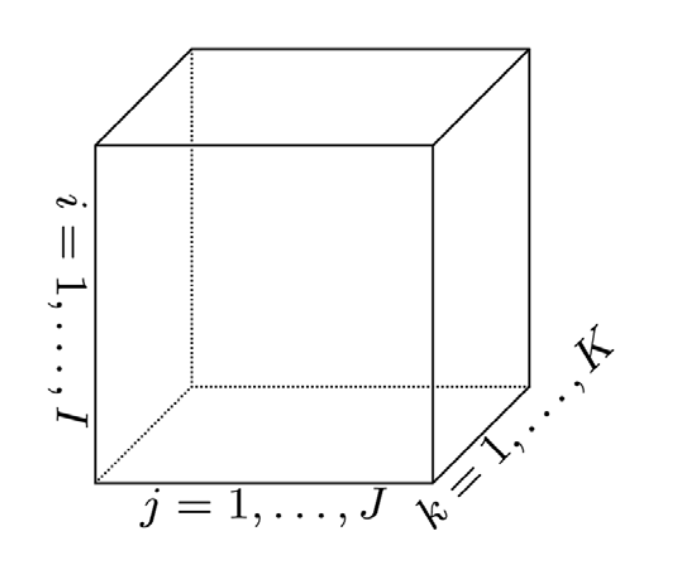
\includegraphics[width=0.3\textwidth]{tensorOrdnung3.png}
	\caption{Tensor dritter Ordnung $\pmb{\mathscr{X}}  \in \mathbb{R}^{I \times J \times K}$ \cite[456]{Kolda}}
	\label{fig:tensorOrdnung3}
\end{figure}

Vorsicht zu haben, gilt es bei den Begriffen Ordnung und Rang bei Tensoren. Es sollte vermieden werden diese Begriffe zu verwechseln. Außerdem sollte man nicht den Begriff des Rangs einer Matrix, mit dem Begriff des Ranges eines Tensors verwechseln. Die Definition des Rangs eines Tensors werden wir hier auslassen, da dies ein überaus schwieriger Begriff ist und es vermieden werden kann in dieser Arbeit damit zu hantieren. Eine ausführliche Erklärung des Begriffs finden Sie in \cite[464]{Kolda}.

\newpage

Um unsere Tensoren zu klassifizieren und charakterisieren, brauchen wir Eigenschaftsbegriffe. Es sei $\pmb{\mathscr{X}}  \in \mathbb{R}^{I_1 \times I_2 \times \dots \times I_N}$ ein Tensor.
\begin{Definition} (Symmetrie)
\begin{itemize}
\item[a)] Den Tensor $\pmb{\mathscr{X}}$ nennt man kubisch genau dann wenn $I_i = I_j$ für alle $i,j$.
\item[b)] Einen kubischen Tensor nennt man supersymmetrisch genau dann wenn die Elemente des Tensors konstant bleiben unter jeglicher Permutation der Indizes.
\item[c)] Einen Tensor nennt man stückweise symmetrisch, wenn die Elemente konstant bleiben unter der Permutation von mindestens 2 Indizes.
\end{itemize}
\end{Definition}

\begin{Definition} (Diagonal) \\
Den Tensor $\pmb{\mathscr{X}}$ nennt man diagonal, wenn
$\, x_{ \, i_1 \,, \, \dots \, , \, i_N \, } \, \neq 0$ genau dann wenn \\ $\, i_1 = \dots = i_N$.
\end{Definition}

\begin{Definition} (Faser) \\
Eine Faser ist das multidimensionale Analog zu Matrixspalten und Matrixzeilen. Wir definieren eine Faser, indem wir jeden Index abgesehen von einem festhalten.
\end{Definition}

Einen Tensor kann man entfalten. Dies impliziert eine Neuordnung der Tensorelemente in eine Matrix.
Wir betrachten nur die sogenannte \textit{mode-n Entfaltung}, da dies die einzig relevante Form der Entfaltung für uns ist.

\begin{Bemerkung} (Entfaltung) \\
Eine mode-n Entfaltung des Tensors $\pmb{\mathscr{X}}$ wird mit $\bold{X}_{(n)}$ geschrieben und ordnet die mode-n Fasern in die Spalten der Ergebnismatrix.
Formal ist es eine Abbildung des Indize N-tupels $(i_1,\dots,i_N)$ auf Matrixindizes $(i_n,j) $
\begin{equation}
j=1+\sum_{\substack{k=1 \\ k \neq n}}^{N} (i_k-1)J_k \text{ mit } J_k = \prod_{\substack{m=1 \\ m \neq n}}^{k-1} I_m
\end{equation}
\end{Bemerkung}

Nun fehlt uns noch eine Tensor Multiplikation um mit der Dekomposition von Tensoren anzufangen. 

\begin{Definition} (n-mode Produkt) \\
Das n-mode Produkt des Tensors $\pmb{\mathscr{X}}$ mit einer Matrix $\bold{U} \in \mathbb{R}^{J \times I_n}$ wird als $\pmb{\mathscr{X}} \times_n \bold{U}$ notiert. Die Ergebnismatrix hat die Größe $I_1 \times \dots I_{n-1} \times J \times I_{n+1} \times \dots I_N$
\begin{equation}
	(\, \pmb{\mathscr{X}} \times_n \bold{U} \, )_{\, i_1 \, \dots \, i_{n-1} \, j \, i_{n+1}\, \dots \, i_N} = \sum_{i_n = 1}^{I_n} x_{\, i_1 \, \dots \, i_N} \, u_{j \, i_n}
\end{equation}
\end{Definition}

\begin{Bemerkung}
Jedes mode-n Produkt kann mit Hilfe von entfaltenen Tensoren äquivalent ausgedrückt werden.
\begin{equation}
\pmb{\mathscr{Y}} = \pmb{\mathscr{X}} \times_n \bold{U} \Longleftrightarrow \bold{Y}_{(n)} = \bold{U} \bold{X}_{(n)}
\end{equation}
\end{Bemerkung}

\subsubsection{Singulärwertzerlegung höherer Ordnung}

Die \textit{Singulärwertzerlegung höherer Ordnung} bzw. \textit{Higher Order Singular Value Decomposition} (HOSVD) oder auch bekannt unter der Tucker Dekomposition ist eine uminterpretierte multidimensionale Hauptkomponentenanalyse. Man versucht durch Hauptachsentransformationen die Korrelation zwischen den verschiedenen Komponenten durch Überführung in eine neue Basis zu minimieren. 
Die HOSVD zerlegt den Tensor in einen sogenannten \textit{Core Tensor} multipliziert mit einer Matrix in jeder Ordnung. 

Allgemein ist die HOSVD des Tensors $\pmb{\mathscr{X}}  \in \mathbb{R}^{I_1 \times I_2 \times \dots \times I_N}$ gegeben durch
\begin{equation}
\pmb{\mathscr{X}}= \pmb{\mathscr{G}} \times_1 \, A^{(1)} \, \dots \, \times_N A^{(N)}
\end{equation}

Man kann äquivalent die HOSVD auch mit entfalteten Tensoren wie folgt angeben
\begin{equation}
\bold{X}_{(n)} = A^{(n)} \, \bold{G}_{(n)} \, ( \, A^{(N)} \, \otimes  \, \dots \, \otimes \, A^{(n+1)} \, \otimes A^{(n-1)} \otimes \dots \otimes \, A^{(1)} \, )^{T}
\end{equation}

\begin{Beispiel} (HOSVD Tensor dritter Ordnung) \\
Es sei $\pmb{\mathscr{X}} \in \mathbb{R}^{I \times J \times K}$.  Dann kann man den Tensor $\pmb{\mathscr{X}}$ zerlegen in 
\begin{equation}
{\pmb{\mathscr{X}}} \approx  \pmb{\mathscr{G}}  \times_1 A \times_2 B \times_3 C 
\end{equation}

wobei $A \in \mathbb{R}^{I \times P}$, $B \in \mathbb{R}^{J \times Q}$ und $C \in \mathbb{R}^{K \times R}$ die Faktormatrizen sind, welche orthogonal sind.
${\cal G}$ bezeichnet den Core Tensor und zeigt wie hoch die Korrelation zwischen den verschiedenen Komponenten ist.

\end{Beispiel}
\begin{figure}[ht]
	\centering
  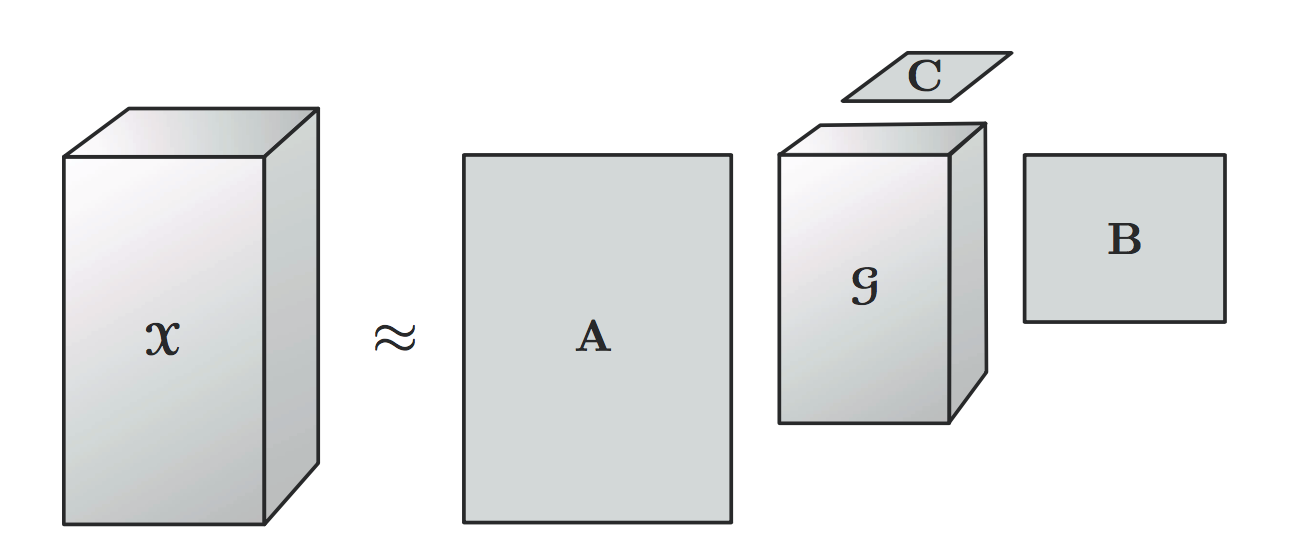
\includegraphics[width=0.6\textwidth]{hosvdTensor.png}
	\caption{HOSVD eines Tensors dritter Ordnung \cite[475]{Kolda}}
	\label{fig:hosvdTensor}
\end{figure}

\newpage
\begin{framed}
\begin{Bemerkung} (Berechnung der HOSVD) \\
Die Berechnung der HOSVD von ${\pmb{\mathscr{X}}}  \in \mathbb{R}^{I_1 \times I_2 \times \dots \times I_N}$ geht wie folgt
\begin{enumerate}
\item Berechne die mode-k Entfaltungen $\bold{X}_{(k)}$ für alle k
\item Berechne die Singulärwertzerlegung $\bold{X}_{(k)}=U_k \Sigma_k V_k^T$ und speichere $U_k$
\item Der Kerntensor ${\pmb{\mathscr{G}}} $ ergibt sich aus der Projektion des Tensors auf die Tensorbasis geformt von den Faktormatrizen  $ \, \{ \, U_k \, \}_{k=1}^{N}$  also $\, \, {\pmb{\mathscr{G}}} ={\pmb{\mathscr{X}}}  \times_{n=1}^{N} \, U_n^T$
\end{enumerate}
\end{Bemerkung}
\end{framed}

Die HOSVD existiert für alle Tensoren. Wie sieht es aber mit der Eindeutigkeit aus? Die HOSVD ist keine eindeutige Zerlegung. Dies führen wir an einem Tensor dritter Ordnung an.

\begin{Beispiel} (Eindeutigkeit der HOSVD) \\
Es seien $U \in \mathbb{R}^{P \times P}$, $V \in \mathbb{R}^{Q \times Q}$  und $W \in \mathbb{R}^{R \times R}$ . Es gilt
\begin{equation}
{\pmb{\mathscr{X}}} = {\pmb{\mathscr{G}}} \times_1 A \times_2 B \times_3 C = ({\pmb{\mathscr{G}}} \times_1 U \times_2 V \times_3 W) \times_1 AU^{-1} \times_2 BV^{-1} \times_3 CW^{-1}
\end{equation}
\end{Beispiel}

In anderen Worten: Wir können den Core Tensor ${\pmb{\mathscr{G}}}$ modifizieren, ohne die Gleichung zu ändern, solange wir das Inverse der Modifizierung auf den zugehörigen Faktormatrizen multiplizieren.

Mit dieser Kenntniss können wir nun zum Beispiel versuchen, soviele Elemente des Kerntensor wie möglich auf Null zu bekommen oder so klein wie möglich zu machen, damit wir bei der späteren Herleitung der Pseudoinversen weniger Probleme bekommen. 

Wir brauchen noch einige Eigenschaften des Kronecker Produkts, die wir uns später für die Berechnung der Pseudoinversen zu Nutze machen wollen.

\begin{Lemma} (Invertieren des Kronecker Produkts) \\
Es seien $A \in \mathbb{R}^{i \times i}$ und $B \in \mathbb{R}^{j \times j}$ invertierbar, so ist auch $(A \otimes B)$ invertierbar. Mit der Inversen
\begin{equation*}
(A \otimes B)^{-1} = A^{-1} \otimes B^{-1}
\end{equation*}
Für die Moore Penrose Pseudoinversen gilt analog
\begin{equation*}
(A \otimes B)^{+} = A^{+} \otimes B^{+}
\end{equation*}
\end{Lemma}

\begin{Lemma} (Matrixprodukt und Kronecker Produkt) \label{lemma:prod} \\
Es seien $A,B,C,D$ Matrizen, deren Matrizenprodukte $AC$ und $BD$ definiert sind, dann gilt
\begin{equation*}
AC \otimes BD = (A \otimes B)(C \otimes D).
\end{equation*}
\end{Lemma}

\begin{Lemma} (Transponieren) \label{lemma:transpose} \\
\begin{equation*}
(A \otimes B)^T=A^T \otimes B^T
\end{equation*}
\end{Lemma}

Dieses Ergebnisse sind entscheidend für die Herleitung der Pseudoinversen. Die theoretische Grundlage ist nun geschaffen. Es ist Zeit sich dem Herz dieser Arbeit zu widmen, nämlich der Tensorstruktur der Elementarsteifigkeitsmatrizen und die Herleitung der Pseudoinversen.





%%%%%%%%%%%%%%%%%%%%%%%%%%%%%%%%%%%%%%%%%%%%%%%%%%%%%%%%%%%%%%%%%%

% Chapter 2
\section{Präkonditionierer für zell-basierte finiten Elemente Operatoren }


%%%%%%%%%%%%%%%%%%%%%%%%%%%%%%%%%%%%%%%%%%%%%%%%%%%%%%%%%%%%%%%%%%


% Chapter 3
\section{Numerische Untersuchungen}


%%%%%%%%%%%%%%%%%%%%%%%%%%%%%%%%%%%%%%%%%%%%%%%%%%%%%%%%%%%%%%%%%%


% Chapter 4
\section{Resultate}


%%%%%%%%%%%%%%%%%%%%%%%%%%%%%%%%%%%%%%%%%%%%%%%%%%%%%%%%%%%%%%%%%%



%Literaturverzeichnis (beginnt auf einer ungeraden Seite)
\newpage
\begin{thebibliography}{Lam00}
\end{thebibliography}
 
% ggf. hier Tabelle mit Symbolen 
% (kann auch auf das Inhaltsverzeichnis folgen)



%%%%%%%%%%%%%%%%%%%%%%%%%%%%%%%%%%%%%%%%%%%%%%%%%%%%%%%%%%%%%%%%%%






\end{document}



